\section{Theoretische Grundlagen}
\subsection{Rutherford-Backscattering-Spectrometry}
Die Rutherford-Backscattering-Spectrometry (RBS) wird zur Untersuchung von dünnen Schichten an Oberflächen verwendet. Dazu werden Ionenstrahlen leichter Kerne wie Helium oder Wasserstoff mit einer kinetischen Energie von $1-4MeV$ auf die Probe geschossen. Dort werden die Ionen an den Kernen elastisch gestreut und so kann ihre Energie in einem Detektor gemessen werden. Meist wird der Detektor so aufgestellt, dass er die Ionen misst, die annähernd unter einem Winkel von $180^\circ$ zur Strahlachse zurückgestreut wurden.

Die Energie der rückgestreuten Teilchen hängt dabei nur von ihrer Anfangsenergie, dem Winkel und den Massen der Stoßpartner ab. Da der Winkel, die Masse des Projektils und die Anfangsenergie des Projektils bekannt ist, kann durch Messung der Energie der gestreuten Ionen die Massenzahlen des Targets bestimmt werden. Im Spektrum ensteht eine Kante maximaler Energie, wo die Teilchen gemessen wurden, die direkt an der Oberfläche gestreut wurden. Die Ionen verlieren in der Probe kontinuierlich Energie durch elastische Stöße mit den Kernen und Anregungen der Hüllenelektronen der Probe. Ionen, die nun tiefer im Target gestreut werden, führen diesen eben beschriebenen Stoßprozess also quasi mit einer geringeren Anfangsenergie durch. Daher gibt es diese kontinuierlich Verteilung von der Kante der maximalen Energie hin zu geringerer Energie.

Bei Kenntnis der Stopping Power, die sich aus den elastischen Kernstößen und den inelastischen Elektronenanregungen zusammen setzt, ist es möglich Tiefeninformationen über die Probe zu erhalten. Beispielsweise kann damit die Dicke einer oder mehrer dünner Schichten bestimmt werden. In diesem Versuch wird sich aber auf die Elementidentifikation beschränkt, weswegen hier nicht näher auf diesen Bereich der RBS eingegangen wird.

\subsection{Der kinematische Faktor}
Der kinematische Faktor oder auch K-Faktor ist definiert durch das Verhältnis der Energie des rückgestreuten Teilchens zur Energie des einfallenden Teilchens:
\begin{equation}
 K = \frac{E_{rueck}}{E_{ein}}
\end{equation}
Er kann somit aus der bekannten Energie $E_{ein}$ und der gemessenen Energie $E_{rueck}$ bestimmt werden. 

Andererseits kann der K-Faktor aus dem elastischen Stoß zweier kugelförmiger Teilchen mit den Massen $m_1$ und $m_2$ hergeleitet werden. Dazu betrachtet man zunächst die drei Gleichungen der Impuls und Energieerhaltung. Angenommen wird, dass sich $m_1$ auf der x-Achse mit der Geschwindigkeit $v$ bewegt und dass sich $m_2$  zu Beginn in Ruhe befinde.
\begin{eqnarray}
 m_1\cdot v^2 & = & m_1\cdot v_1^2 + m_2\cdot v_2^2\label{energie}\\
 m_1\cdot v & = & m_1\cdot v_1\cdot \cos \theta + m_2\cdot v_2\cdot \cos \phi\label{impuls1}\\
 0 &=& m_1\cdot v_1\cdot \sin \theta - m_2\cdot v_2\cdot\sin \phi\label{impuls2}
\end{eqnarray}

Dabei ist $\theta$ der Winkel unter dem das Projektil zurück gestreut wird und $\phi$ der Winkel unter dem sich der Kern nach dem Stoß bewegt. Nun wird zunächst der Winkel $\phi$ eliminiert, indem die Gleichungen \ref{impuls1} und \ref{impuls2} quadriert und addiert werden:
\begin{equation}
 m_1^2\cdot v^2- 2m_1^2\cdot v\cdot v_1\cdot \cos \theta + m_1^2\cdot v_1^2\cdot\cos^2\theta + m_1^2\cdot v_1^2\cdot \sin^2\theta = m_2^2\cdot v_2^2
\end{equation}
Weitere Vereinfachungen und $m_2^2\cdot v_2^2=m_2m_1(v^2-v_1^2)$ aus Gleichung \ref{energie}  ergeben:
\begin{equation}
 m_1^2\cdot v^2- 2m_1^2\cdot v\cdot v_1\cdot \cos \theta + m_1^2\cdot v_1^2= m_2m_1(v^2-v_1^2)
\end{equation}
Mit den Substitutionen $\sqrt{K}=\frac{v_1}{v}$ und $A=\frac{m_2}{m_1}$ erhält man die quadratische Bestimmungsgleichung für $\sqrt{K}$:
\begin{equation}
 \sqrt{K}^2 - \frac{2\cos\theta}{A+1}\sqrt{K} - \frac{A-1}{A+1}=0
\end{equation}
Die beiden Lösungen für $\sqrt{K}$ sind dann
\begin{equation}
  \sqrt{K}=\frac{\cos\theta}{A+1}\pm\sqrt{\frac{\cos^2 \theta}{(A+1)^2}+\frac{A-1}{A+1}}, 
\end{equation}
wobei die Lösung mit dem Minuszeichen verworfen werden kann, da für $A>1$ das Verhältnis der Geschwindigekeiten $\sqrt{K}$ nicht negativ werden soll. Resubstituiert und quadriert folgt damit abschließend:
\begin{equation}
 K = \left\{ \frac{\cos \theta+ \sqrt{\frac{m_2^2}{m_1^2}-\sin^2\theta}}{\frac{m_2}{m_1}+1} \right\}^2,
\end{equation}
bzw.
\begin{equation}
 K = \left\{ \frac{m_1\cdot\cos \theta+ \sqrt{m_2^2-m_1^2\cdot\sin^2\theta}}{m_2+m_1} \right\}^2.
\end{equation}
Damit ist der K-Faktor auch hier wieder das Verhältnis von rückgestreuter Energie zu einlaufender Energie des Projetils.

Nun kann der K-Faktor für alle möglichen Elemente und He$^+$-Projektilen unter einem bestimmten Winkel berechnet und tabelliert werden. Dadurch ist ein komfortables Finden der passenden Elemente möglich, nachdem der K-Faktor experimentell bestimmt wurde.

\subsection{Der Van-de-Graaff-Beschleuniger}
Zur Beschleunigung der Helium-Ionen wird ein Van-de-Graaff-Beschleuniger verwendet. Dieser arbeitet mit dem Prinzip des Van-de-Graaff-Generators, der durch ein mechanisches angetriebenes Band positive Ladungen erzeugt.
\begin{figure}[htbp]  
     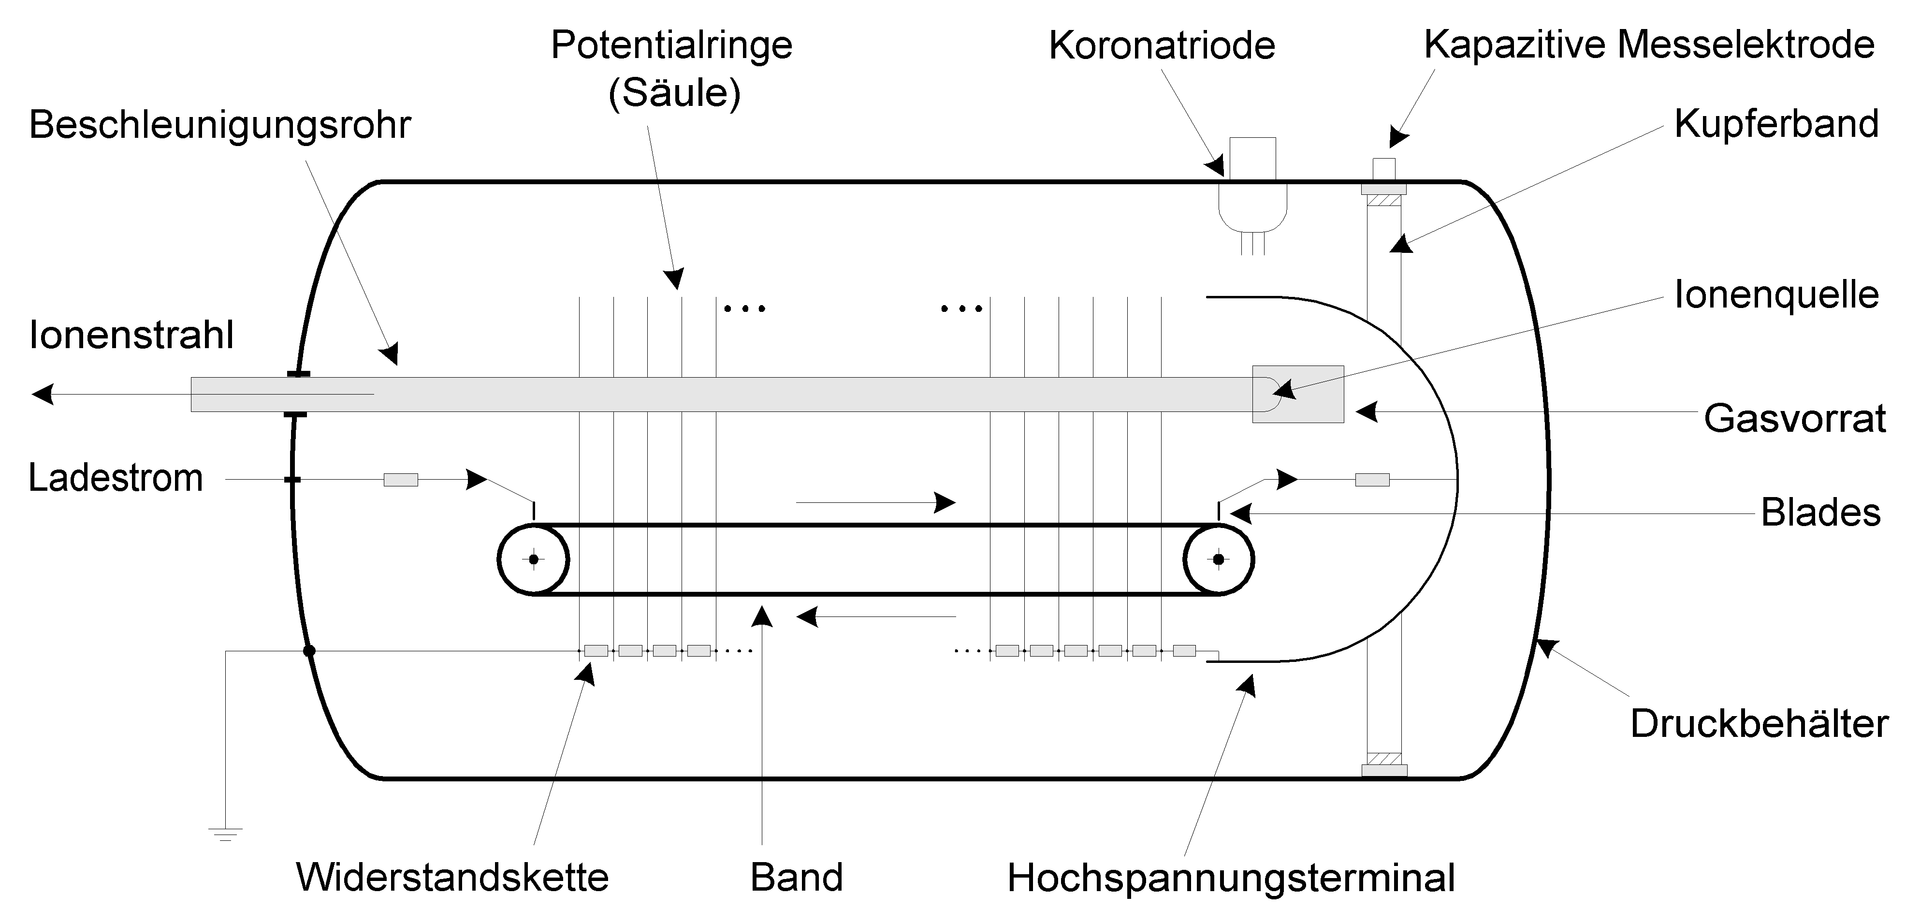
\includegraphics[width=0.99\textwidth]{van_de_graaff.png}
  \caption{Prinzipieller Aufbau eines Van-de-Graaff-Beschleunigers \cite{van_de_graaff}}
  \label{van_de_graaff}
\end{figure}

Wie man in Abbildung \ref{van_de_graaff} erkennen kann, werden die positiven Ladungen dann über Blades auf ein Hochspannungsterminal geleitet. Es wird so eine Hochspannung von mehreren Megavolt erzeugt, über Spannungsteiler auf die Potentialringe, die sogenannte Säule, aufgeteilt wird. Die Ionen aus der Ionenquelle werden somit entlang des Ionenstrahls gleichmäßig beschleunigt.

Das Generatorsystem ist mit einem Gas besonders hoher Durchschlagsfestigkeit gefüllt, SF$_6$ oder XeCO$_2$, da die maximale Terminalspannung hauptsächlich von der Durchschlagsfestigkeit des umgebenden Mediums abhängt. Die kapazitive Messelektrode misst Schwankungen in der Spannung und so kann die Koronatriode durch Aufbringung von negativen Ladungen auf das Hochspannungsterminal die Spannung stabilisieren. Es wird so eine Stabilität der Strahlenergie von $0,1\%$ erreicht.




